\documentclass[presentation]{beamer}
%\documentclass[handout]{beamer}
\usetheme{Frankfurt}
\usecolortheme{seahorse}

\usepackage{amssymb}
\usepackage{amsmath}
\usepackage{graphicx}
\usepackage{subcaption}

\usepackage{tikz}
\usetikzlibrary{graphdrawing,graphs} 
\usegdlibrary{layered}
\usegdlibrary{force}
\usegdlibrary{trees}

\usepackage{hyperref}

\begin{document}

\title{Using Time Series Models for Defect Prediction in Software Release Planning}
\author{James Tunnell \\
Central Washington University \\
Computational Science Program}

\begin{frame}
\titlepage
\end{frame}

\begin{frame}
\frametitle{Outline}
\tableofcontents[hideallsubsections] 
\end{frame}

\section{Introduction}

\begin{frame}
\begin{center}
\Large{Introduction}
\end{center}
\end{frame}

\subsection{Release Planning}

\begin{frame}[t]
\frametitle{Release Planning Objectives}
\begin{itemize}
\item{Two primary objectives of software release planning are:
  \begin{itemize}
    \item{Improving functionality}
    \item{Maintaining quality}
  \end{itemize}}
  \item{Both of these objectives are constrained by limits on development time and cost.}
\end{itemize}
\end{frame}

\subsection{Quality Control}

\begin{frame}[t]
\frametitle{Quality Control}
\begin{itemize}
  \item{Software defects (bugs) are inevitable}
  \item{Sufficient time should be available to ensure good quality (by testing and bug-fixing)}
  \item{Otherwise, there is a risk of
    \begin{itemize}
    \item{Low quality (failure to meet objective)}
    \item{Schedule slip (failure to respect constraint)}
    \end{itemize}
  }
  \item{This quality control (QC) time can be allowed for by limiting the scope of work in the planned release}
\end{itemize}
\end{frame}

\begin{frame}[t]
\frametitle{Quality Control (cont'd)}
\begin{itemize}
  \item{To support release planning, QC time can be estimated}
  \item{Assumption: QC time depends (at least partly) on the number of software defects introduced}
  \item{Then, a basis for estimating QC time would be the predicted number of defects}
\end{itemize}
\end{frame}

\subsection{Defect Prediction}

\begin{frame}[t]
\frametitle{Defect Prediction}
\begin{itemize}
  \item{Approaches to defect prediction tend to focus on either
    \begin{itemize}
    \item{Code analysis
      \begin{itemize}
      \item{Lines of code}
      \item{Number of decisions}
      \item{Code churn}
      \end{itemize}
    }
    \item{Historical information
      \begin{itemize}
      \item{Regression analysis}
      \item{Time series modeling}
	  \end{itemize}
	}
    \end{itemize}
  }
  \item{A multivariate time series model with exogenous inputs was chosen}
\end{itemize}
\end{frame}

\section{Motivation}

\begin{frame}
\begin{center}
\Large{Motivation}
\end{center}
\end{frame}

\subsection{Release Plan Optimization}

\begin{frame}[t]
\frametitle{Release Plan Optimization}
\begin{itemize}
  \item{A release plan is formed by selecting features and improvements to work on}
  \item{Release plans can be compared by the expected revenue they will generate}
  \item{This optimization problem is posed as The Next Release Problem (NRP)}
\end{itemize}
\end{frame}

\begin{frame}[t]
\frametitle{Release Plan Optimization (cont'd)}
\begin{itemize}
  \item{The NRP is an abstract optimization problem}
  \item{In practice, QC time should be considered to ensure constraints are respected}
  \item{With the help of a defect prediction model, QC time can be estimated}
  \item{In this context, release plans are being compared}
  \item{For a defect prediction model to be useful, it should depend in some way on the basic elements of the release plan (planned new features and improvements)}
\end{itemize}
\end{frame}

\subsection{Explanatory Model}

\begin{frame}[t]
\frametitle{Explanatory Model}
\begin{itemize}
\item{Assumption: the number of defects in the future depends on more than just the number of defects in the past}
\item{A defect prediction model that depends only on previous numbers of defects is not explanatory}
\item{Such a non-explanatory model would always predict the same number of defects}
\end{itemize}

\begin{figure}[htbp]
\begin{center}
\tikz[nodes={text height=1em, text depth=.2em, draw=black!20, thick, fill=white, font=\small}, rounded corners, semithick]
  \graph[layered layout, level distance = 1cm, sibling sep = 1em]{
    "Release Plan 1" -> "Explanatory Model";
    "Release Plan 2" -> "Explanatory Model";
    "...." -> "Explanatory Model";
    "Release Plan N" -> "Explanatory Model";
    "Explanatory Model" -> "Predicted Defects";
  };
\caption{A non-explanatory model.}
\end{center}
\end{figure}
\end{frame}


\begin{frame}[t]
\frametitle{Explanatory Model (cont'd)}
\begin{itemize}
\item{A model could also depend on the key factors of a release plan}
\item{This would be an explanatory model structure}
\item{Such a model can potentially predict a different number of defects for every release plan}
\end{itemize}

\begin{figure}[htbp]
\begin{center}
\tikz[nodes={text height=1em, text depth=.2em, draw=black!20, thick, fill=white, font=\small}, rounded corners, semithick]
  \graph[layered layout, level distance = 1cm, sibling sep = 1em]{
    "Release Plan 1" -> "Explanatory Model";
    "Release Plan 2" -> "Explanatory Model";
    "...." -> "Explanatory Model";
    "Release Plan N" -> "Explanatory Model";
    "Explanatory Model" -> "Predicted Defects 1";
    "Explanatory Model" -> "Predicted Defects 2";
    "Explanatory Model" -> "...";
    "Explanatory Model" -> "Predicted Defects N";
  };
\caption{An explanatory model.}
\end{center}
\end{figure}
\end{frame}

\section{Related Work}

\begin{frame}
\begin{center}
\Large{Related Work}
\end{center}
\end{frame}

\subsection{Code Analysis}

\begin{frame}[t]
\frametitle{Defect Prediction using Code Analysis}
\begin{itemize}
\item{Approaches using code analysis:
  \begin{itemize}
  \item{Akiyama used lines of code (LOC), number of decisions, and the number of subroutine calls \cite{1971_akiyama}}
  \item{Gafney also used LOC \cite{1984_gaffney_estimating}}
  \item{Henry and Kafura use information taken from design documents \cite{1984_henry_evaluation}}
  \item{Nagappan and Ball use relative code churn (lines modified) \cite{2005_nagappan_codechurn}}
  \end{itemize}
}
\item{These approaches all depend on specific design or implementation information}
\item{This information is not available at the release planning stage}
\end{itemize}
\end{frame}

\subsection{Historical Information}

\begin{frame}[t]
\frametitle{Defect Prediction using Historical Information}
\begin{itemize}
\item{Approaches using historical information:
  \begin{itemize}
  \item{Li et al. extrapolate parameters of a regression model \cite{2004_li_emperical_eval}}
  \item{Singh et al. use an ARIMA time series model \cite{2010_singh_predicting}}
  \end{itemize}
}
\item{Both approaches are non-specific to design or implementation}
\item{However, neither approach is explanatory}
\end{itemize}
\end{frame}


\section{Time Series Modeling}

\begin{frame}
\begin{center}
\Large{Time Series Modeling}
\end{center}
\end{frame}


\subsection{Time Series}

\begin{frame}[t]
\frametitle{Time Series }
\begin{itemize}
\item{A time series is a collection of observations that occur in order}
\item{The process underlying a time series is assumed to be stochastic (non-deterministic)}
\item{Each observation might depend on one or more previous observations}
\item{This dependence is termed autocorrelation}
\end{itemize}
\end{frame}

\subsection{Autoregressive Models}

\begin{frame}[t]
\frametitle{Autoregressive Models}
\begin{itemize}
\item{A basic autoregressive (AR) model is a linear combination of previous values}
\item{A white noise term accounts for stochastic fluctuation}
\item{An $AR(p)$ model for predicting a value X at time t is
\begin{equation}
X_t=c+\sum_{i=1}^{p}{\phi_t X_{t-1}+\epsilon_t}
\end{equation}
where $\phi_1, \phi_2, ..., \phi_p$ are the $p$ parameters, $c$ is a constant, and $\epsilon_t$ is the white noise term}
\end{itemize}
\end{frame}

\begin{frame}[t]
\frametitle{Autoregressive Models (cont'd)}
\begin{itemize}
\item{Extending the AR model to be multivariate results in a Vector AR (VAR) model}
\item{This model can support time series for defect count, improvements, and new features}
\end{itemize}
\end{frame}

\subsection{Endogeneity and Exogeneity}

\begin{frame}[t]
\frametitle{Endogeneity and Exogeneity}
\begin{itemize}
\item{Under a VAR model, the behavior of each time series is explained by both
its own past values and the past values of the other time series}
\item{This makes the variables endogenous}
\item{An alternative is that a time series is only used to explain other time series}
\item{This type of explanatory variable is called exogenous, and could be considered an input}
\item{Exogenouse variables are not explained by the model}
\end{itemize}
\end{frame}

\begin{frame}[t]
\frametitle{Endogeneity and Exogeneity (cont'd)}
\begin{itemize}
\item{The desired model does not need to explain features and improvements}
\item{Instead, these are used to explain defects}
\item{Planned features and improvements can be made exogenous}
\item{By also considering exogenous variables, a VAR model would become a
VARX model}
\end{itemize}
\end{frame}

\subsection{Stationarity and Trends}

\begin{frame}[t]
\frametitle{Stationarity}
\begin{itemize}
\item{A stationary time series has time-invariant statistics}
\item{The time series models so far require time series to be stationary}
\item{Differencing a non-stationary series may produce a stationary series}
\item{Stationary can determined by testing for trends}
\end{itemize}
\end{frame}

\begin{frame}[t]
\frametitle{Deterministic Trends}
\footnotesize{
\begin{itemize}
\item{A time series with a deterministic trend has a non-constant mean}
\item{The time series movements will generally follow the deterministic function}
\item{Fluctuations above or below this function are non-permanent}
\item{Such a time series is said to be stationary around a deterministic trend}
\end{itemize}
}
\begin{figure}[htbp]
\begin{center}
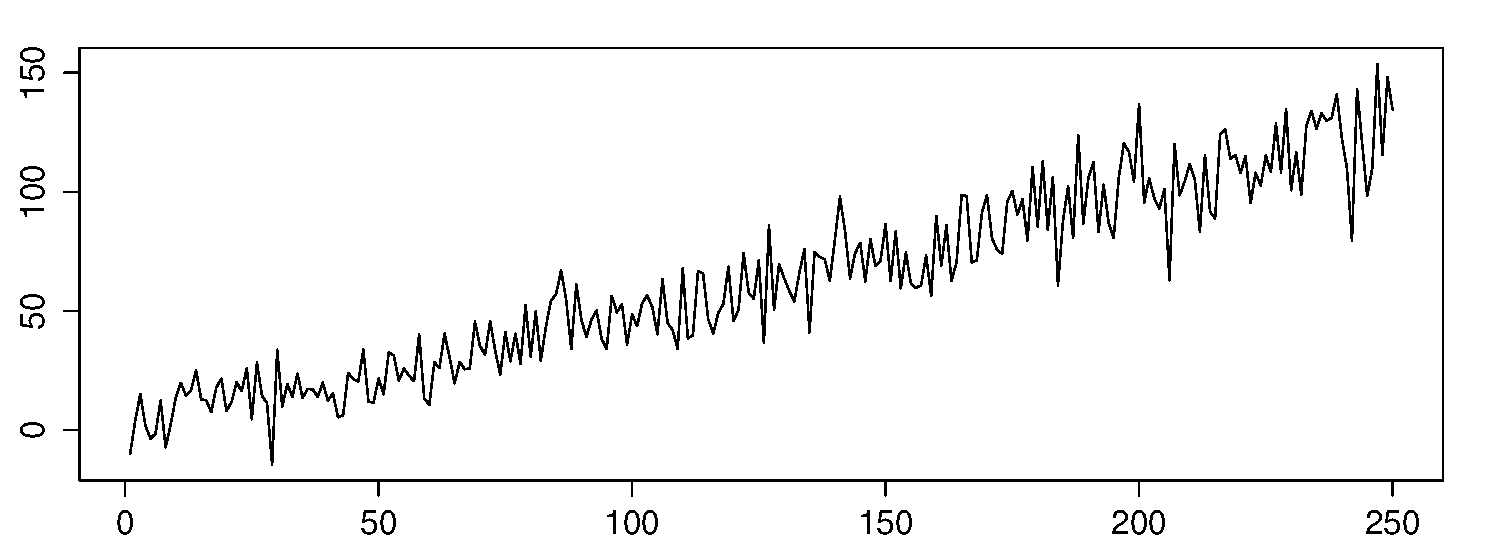
\includegraphics[width=\textwidth]{assets/deterministic_trend.eps}
\caption{Time series with a deterministic trend.}
\end{center}
\end{figure}
\end{frame}


\begin{frame}[t]
\frametitle{Stochastic Trends}
\footnotesize{
\begin{itemize}
\item{A stochastic trend shows permanent effects due to random variations}
\item{A series with stochastic trend will not necessarily fluctuate only close to the area of a deterministic function}
\item{A time series with stochastic trend is non-stationary}
\item{Differencing can be used to remove a stochastic trend}
\end{itemize}
}
\vspace{-.2cm}
\begin{figure}[htbp]
\begin{center}
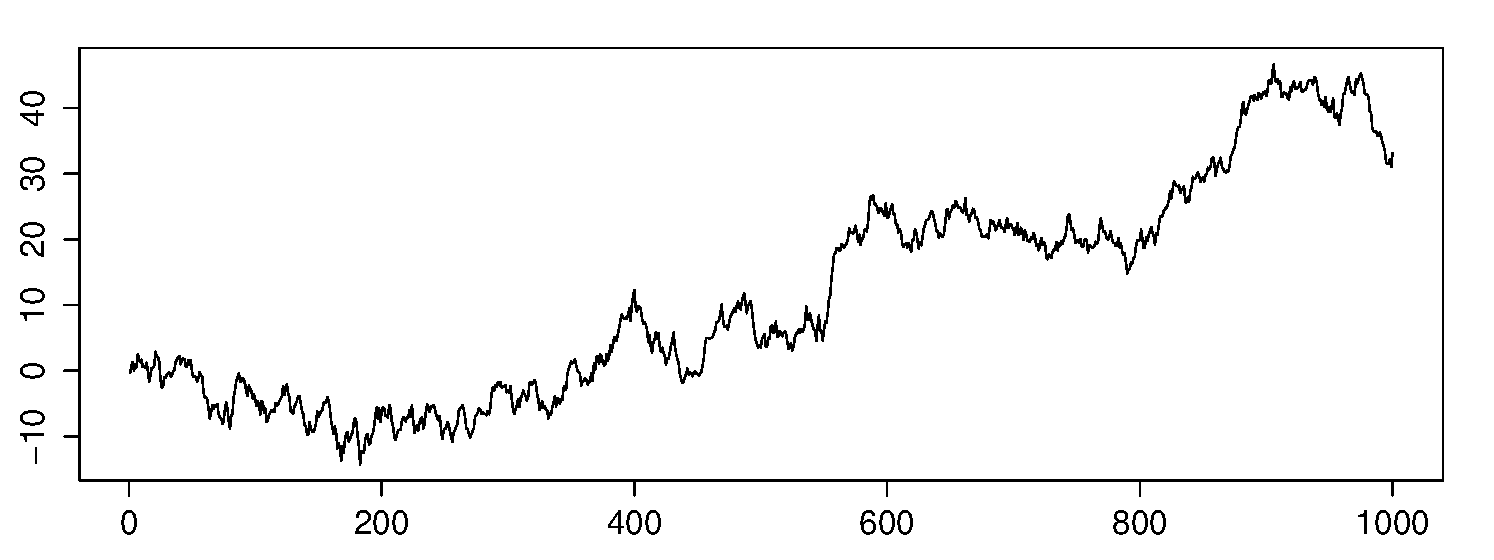
\includegraphics[width=\textwidth]{assets/stochastic_trend.eps}
\caption{Time series with a stochastic trend.}
\end{center}
\end{figure}
\end{frame}

\subsection{Stationarity Testing}

\begin{frame}[t]
\frametitle{Stationarity Testing}
\footnotesize{
\begin{itemize}
\item{A pure AR model of a time series with stochastic trend contains a unit root \cite{franses1998time}}
\item{Testing for the presence of a unit root can therefore be used to test for non-stationarity}
\item{A unit-root test starts with the null hypothesis that an AR model has a unit root}
\item{The alternative hypothesis is that an AR model of the time series does not have a unit root}
\item{Next, a test statistic is measured}
\item{If the test statistic is below the chosen significance level, the null hypothesis is rejected}
\item{Rejecting the null hypothesis provides reason to accept the alternative hypothesis}
\item{The Augmented Dickey Fuller (ADF) test is commonly used for unit root testing}
\end{itemize}
}
\end{frame}

\begin{frame}[t]
\frametitle{Stationarity Testing (cont'd)}
\footnotesize{
\begin{itemize}
\item{On the other hand is a stationarity test}
\item{This test starts with the null hypothesis that a time series is stationary around a deterministic trend}
\item{If the test statistic is above some significance level, this shows that the null hypothesis can be accepted}
\item{Then the time series should be considered stationary}
\item{The Kwiatkowski-Phillips-Schmidt-Shin (KPSS) test can be applied for testing stationarity.}
\end{itemize}
}
\end{frame}

\section{Modeling Methodology}

\begin{frame}
\begin{center}
\Large{Modeling Methodology}
\end{center}
\end{frame}

\section{Data Methodology}

\begin{frame}
\begin{center}
\Large{Data Methodology}
\end{center}
\end{frame}

\note{In this section, the data source and data collection method are detailed. Then, the method of preparing data for the modeling phase is presented.}

\section{References}

\begin{frame}[allowframebreaks]{References}
\begin{center}
\bibliography{references}
\bibliographystyle{abbrv}
\end{center}
\end{frame}

\end{document}
